\documentclass[12pt,a4paper]{article}
\usepackage{pgf}
% \usepackage[condensed,math]{kurier}
% \usepackage[T1]{fontenc}
\usepackage{svg}
\usepackage{tikz}
\usepackage{stanli}
\usepackage{afterpage}
\usepackage{multirow}
\usepackage{subfig}
\usepackage{pgfpages}
\usepackage{svg}
\usepackage{rotating}

%\usepackage{times}


\pgfpagesdeclarelayout{boxed}
{
	\edef\pgfpageoptionborder{0pt}
}
{
	\pgfpagesphysicalpageoptions
	{%
		logical pages=1,%
	}
	\pgfpageslogicalpageoptions{1}
	{
		border code=\pgfsetlinewidth{2pt}\pgfstroke,%
		border shrink=\pgfpageoptionborder,%
		resized width=.9\pgfphysicalwidth,%
		resized height=.9\pgfphysicalheight,%
		center=\pgfpoint{.5\pgfphysicalwidth}{.5\pgfphysicalheight}%
	}%
}

\pgfpagesuselayout{boxed}


% Language setting
% Replace `english' with e.g. `spanish' to change the document language
\usepackage[english]{babel}

% Set page size and margins
% Replace `letterpaper' with `a4paper' for UK/EU standard size
\usepackage[a4paper,top=2cm,bottom=1.5cm,left=1.5cm,right=1.5cm,marginparwidth=1.75cm]{geometry}

% Useful packages
\usepackage{amsmath}
\usepackage{graphicx}
\usepackage[colorlinks=true, allcolors=blue]{hyperref}

\title{}
\author{}
\date{}

\begin{document}
	
	\newcommand{\subf}[2]{%
		{\small\begin{tabular}[t]{@{}c@{}}
				#1\\#2
		\end{tabular}}%
	}
	
	\begin{titlepage}
		\begin{center}
			\vspace*{3cm}
			
			\Huge
			\textbf{Simulation and Models: Report}
			
			\vspace{0.3cm}
			\Huge
			Project 1
			
			\vspace{0.8cm}
			\large
			
			%INSTRUCTED BY: MRS. A.A.S.KAUSHLYA
			
			
			\vspace{0.5cm}
			\LARGE
			
			
			\vspace{1.5cm}
			
			\textbf{}
            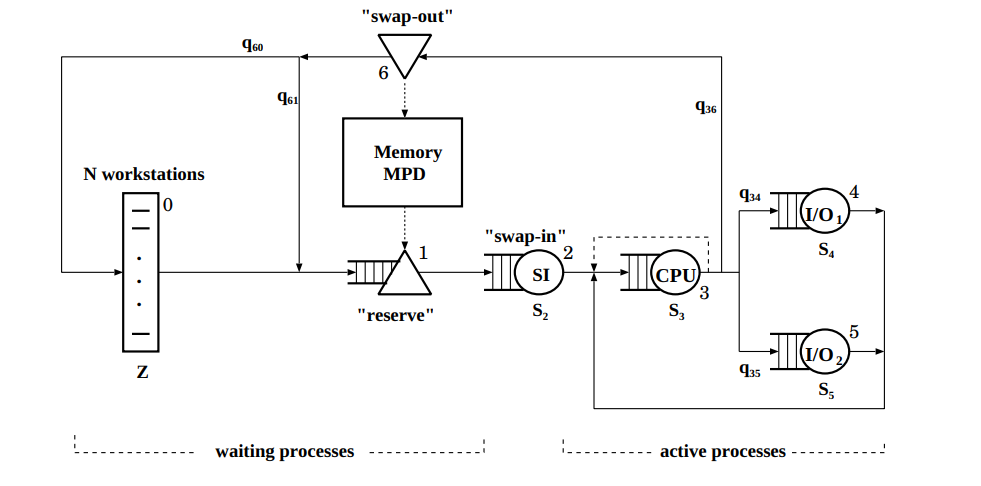
\includegraphics[width=0.8\textwidth]{Images/model.png}
			
			\vfill
			
			
			
			\vspace{0.8cm}
			
			
			
			\Large
			
			
			
			
		\end{center}
		\Large
		\begin{tabbing}
			\hspace*{1em}\= \hspace*{8em} \= \kill % set the tabbings
			\> Name:\>  \textbf{Matteo Ielacqua} \\
			\> Date of Per: \> 01.2024\\
			\> Date of Sub: \> 01.2024
		\end{tabbing}
		
	\end{titlepage}
	
	
	
	\section{Description of the System}
	

    \section{BottleNeck Analysis}
    In order to start the analysis , let's show here the simplified model 
    used to conduct the validation.
    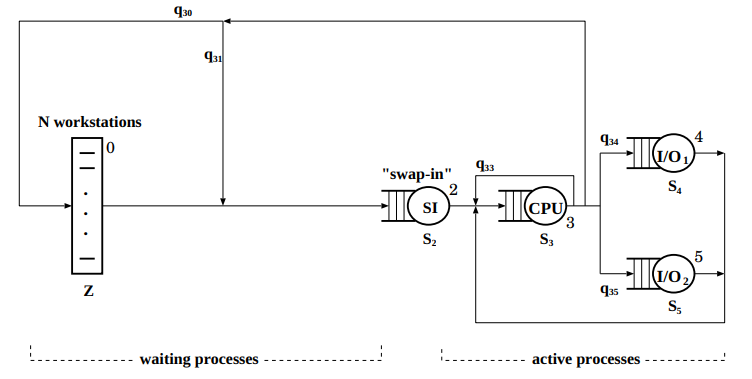
\includegraphics[width=0.8\textwidth]{Images/simplified_model.png}
    \\And summarize some data:
    \begin{displaymath}
        \begin{aligned}
        S_2 = 210ms && S_3= 2.7ms && S_4 = 40ms && S_5=180ms\\
        q_{3,0}= 0.4&& q_{3,1}=0.6 && q_{3,3} = 0.9 && q_{3,4}= 0.065\\
        && q_{3.5}= 0.025 && q_{3,6}=0.01 && 
        \end{aligned}
    \end{displaymath}
    From this data we can witness that this may be a good approximation, considering that
    a process has a probability of 0.9 to return back with a mean service time of 2.7, 
    we know from the original model that clients have a mean service time of 27 ms with 
    a fixed cpu slice time of 2.7 ms, so we expect a customer to be rescheduled in the cpu 
    almost another 9 times since the first one it is scheduled. \\

    From the previous data we can extract this matrix 
    \begin{displaymath}
        \begin{bmatrix}
            0 && 1 && 0 && 0 && 0 \\
            0 && 0 && 1 && 0 && 0 \\
            0.004 && 0.006 && 0.9 && 0.065 && 0.025 \\
            0 && 0 && 1 && 0 && 0 \\
            0 && 0 && 1 && 0 && 0 \\
        \end{bmatrix}
        \begin{bmatrix}
            0 && 0 && 0.004 && 0 && 0 \\
            1 && 0 && 0.006 && 0 && 0 \\
            0 && 1 && 0.9 && 1 && 1 \\
            0 && 0 && 0.065 && 0 && 0\\
            0 && 0 && 0.025 && 0 && 0
        \end{bmatrix}
    \end{displaymath}

    From which we can extract the following system of equations 
    \begin{displaymath}
        \begin{cases}
            V_0=0.004V_3\\
            V_2=V_0+0.004V_3\\
            V_3=V_2+0.9V_3+V_4+V_5\\
            V_4=0.065V_3
            V_5= 0.025V_3
        \end{cases}
    \end{displaymath}
    with the additional equation $V_0=1$. Resolving this system lead to the computation 
    all Vs 
    \begin{displaymath}
        \begin{cases}
            V_0=1 \\
            V_3=250\\
            V_2=2.5\\
            V_4=16.25\\
            V_5=6.25
        \end{cases}
    \end{displaymath}

    From this computes Vs is possible to detect which of the station is the bottleneck of the system
    by considering that $VbS_b= \max_i\{V_iS_i\}$, so let's compute all $V_iS_i$ and find 
    the greater one. 

    \begin{displaymath}
        \begin{aligned}
            V_2S_2= 525ms && V_3S_3=675ms && V_4S_4=650ms && V_5S_5= 1125ms
        \end{aligned}
    \end{displaymath}
    from this calculation we can say that $V_bS_b=V_5S_5=1125ms$ and so , station 5 (IO2) is 
    our bottleneck. Let's extract some additional information, as the total cycle time when $N=1$ ,i.e Y(1) 
    \begin{displaymath}
        D=\sum_{i=1}^{N}D_i=\sum_{i=1}^{N}V_iS_i=2975ms
    \end{displaymath}
    Thus we can also calculate the saturation point $N^*$ of this system, after which we can expect
    the total response time will increase. 
    \begin{displaymath}
        N^*=\frac{Y(1)}{V_bS_b}=\frac{D}{V_bS_b}=\frac{2975ms}{1125ms}=2.64
    \end{displaymath}

    \end{document}